%% !TEX root = manual.tex

\chapter{Topologies}
\label{chapter:topologies}


The torus topology is straightforward and easy to understand.
Here we introduce the basics of other topologies within SST that are more complex and require extra documentation to configure properly.
These are generally higher-radix or path-diverse topologies like fat tree, dragonfly, and flattened butterfly.  
As noted in \ref{sec:tutorial:topology}, a more thorough and excellent discussions of these topologies is given in ``High Performance Datacenter Networks'' by Dennis Abts and John Kim.

\section{Topology Query Utility}
\label{sec:topologyQuery}
Understanding topology inputs and geometries can sometimes be challenging.
\sstmacro provides an executable for testing topology inputs and doing example coordinate computations.
After making and installing, an executable \inlineshell{sstmac_top_info} will appear in the \inlineshell{bin} folder.
The invocation of \inlineshell{sstmac_top_info} is exactly the same as the main \inlineshell{sstmac} executable.
For the example parameter file named \inlineshell{machine.ini}:

\begin{ViFile}
topology.name = fattree
topology.geometry = 4 3
\end{ViFile}

we run

\begin{ShellCmd}
bin> sstmac_top_info -f machine.ini
\end{ShellCmd}
which produces the output

\begin{ViFile}
Number of nodes:         81
Number of leaf switches: 27
Number of switches:      94
\end{ViFile}

detailing the produced geometry.  Here the fat tree has a total of 94 switches, 27 of which are ``leaf'' switches directly connected to compute nodes.
The output is followed by the prompt

\begin{ShellCmd}
NextInput: 
\end{ShellCmd}

One can either enter a single number (switch ID) or set of coordinates.
If given a switch ID, the coordinates are computed.
If coordinates are given, the switch ID is computed.

\begin{ShellCmd}
NextInput: 32
Switch ID maps to coordinates [ 2 0 1 2 ]
NextInput: 2 0 1 2
Coordinates map to switch ID 32
\end{ShellCmd}

The program is just exited with Ctrl-C.
The meaning of the above coordinates is detail below for fat tree (Section \ref{sec:tutorial:fattree}).


% !TEX root = manual.tex
\section{Torus}
\label{subsec:tutorial:hypercube}

The torus is the simplest topology and fairly easy to understand.
We have already discussed basic indexing and allocation as well as routing.
More complicated allocation schemes with greater fine-grained control can be used such as the
coordinate allocation scheme (see hypercube below for examples) and the node ID allocation scheme (see fat tree below for examples).
More complicated Valiant and UGAL routing schemes are shown below for hypercube and dragonfly,
but apply equally well to torus.

For torus we illustrate here the Cartesian allocation for generating regular Cartesian subsets.
For this, the input file would look like 

\begin{ViFile}
topology {
 name = torus
 geometry = 4 4 4
}
node {
 app1 {
  launch_cmd = aprun -n 8
  indexing = block
  allocation = cartesian
  cart_sizes = 2 2 2
  cart_offsets = 0 0 0
 }
}
\end{ViFile}

This allocates a 3D torus of size 4x4x4.
Suppose we want to allocate all 8 MPI ranks in a single octant?
We can place them all in a 2x2x2 3D sub-torus by specifying the size of the sublock 
(\inlineshell{cart_sizes}) and which octant (\inlineshell{cart_offsets}).
This applies equally well to higher dimensional analogs.
This is particularly useful for allocation on Blue Gene machines
which always maintain contiguous allocations on a subset of nodes.

This allocation is slightly more complicated if we have multiple nodes per switch.
Even though we have a 3D torus, 
we treat the geometry as a 4D coordinate space with the 4th dimension referring to nodes connected to the same switch, 
i.e. if two nodes have the 4D coordinates [1 2 3 0] and [1 2 3 1] they are both connected to the same switch.
Consider the example below:

\begin{ViFile}
topology {
 name = torus
 geometry = 4 4 4
 concentration = 2
}
app1 {
 launch_cmd = aprun -n 8
 indexing = block
 allocation = cartesian
 cart_sizes = 2 2 1 2
 cart_offsets = 0 0 0 0
}
\end{ViFile}

We allocate a set of switches across an XY plane (2 in X, 2 in Y, 1 in Z for a single plane).
The last entry in \inlineshell{cart_sizes} indicates that both nodes on each switch should be used.



% !TEX root = manual.tex
\section{Hypercube}
\label{subsec:tutorial:hypercube}

Although never used at scale in a production system, the generalized hypercube is an important topology to understand, particularly for flattened butterfly and dragonfly.
The (k,n) generalized hypercube is geometrically an N-dimensional torus with each dimension having size k (although dimension sizes need not be equal).
Here we show a (4,2) generalized hypercube (Figure \ref{fig:topologies:hypercubeConnected}).  This would be specified in SST as:

\begin{ViFile}
topology.name = hypercube
topology.geometry = 4 4 
\end{ViFile}
indicating size 4 in two dimensions. 

While a torus only has nearest-neighbor connections, a hypercube has full connectivity within a row and column (Figure \ref{fig:topologies:hypercubeConnected}).
Any switches in the same row or same column can send packets with only a single hop.

\begin{figure}[h!]
\centering
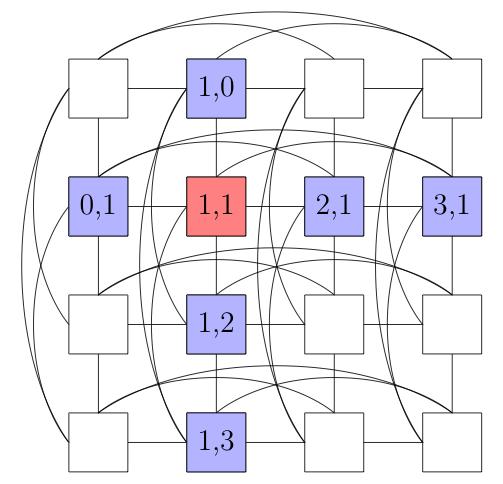
\includegraphics[width=0.5\textwidth]{figures/tikz/hypercube/hypercube_connected.png}
\caption{Hypercube with links and connections within a row/column}
\label{fig:topologies:hypercubeConnected}
\end{figure}

This extra connectivity leads to greater path diversity and higher radix switches.
The cost tradeoff is that each link has lower bandwidth than a torus. 
Whereas a torus has a few fat links connecting switches, a hypercube has many thin links.
A hypercube can have more dimensions and be asymmetric, e.g.

\begin{ViFile}
topology.name = hypercube
topology.geometry = 4 5 6
\end{ViFile}

where now we have full connections within horizontal rows, horizontal columns, and vertical columns.
Here each switch has radix 12 (3 connections in X, 4 connections in Y, 5 connections in Z). 

\subsection{Allocation and indexing}
\label{subsec:hypercube:allocation}

A hypercube has the same coordinate system as a torus. For example, to create a very specific, irregular allocation on a hyerpcube:

\begin{ViFile}
node {
 app1 {
  launch_cmd = aprun -n 5
  indexing = coordinate
  allocation = coordinate
  coordinate_file = coords.txt
 }
}
\end{ViFile}
and then a coordinate file named \inlineshell{coords.txt}

\begin{ViFile}
5 2
0 0
0 1
1 1
2 0
3 3
\end{ViFile}
The first line indicates 5 entries each with 2 coordinates.
Each line then defines where MPI ranks 0-4 will be placed

\begin{figure}[h!]
\centering
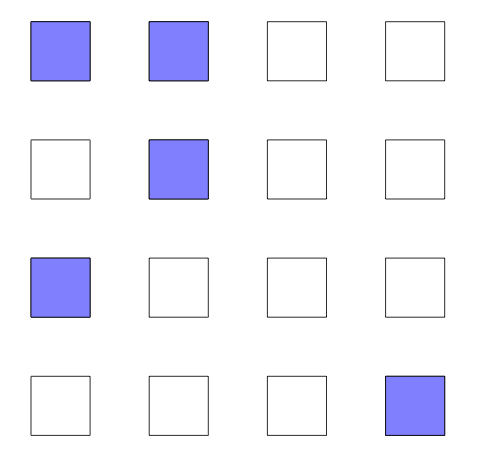
\includegraphics[width=0.5\textwidth]{figures/tikz/hypercube/hypercube_allocation.png}
\caption{Hypercube allocation for given set of coordinates}
\label{fig:topologies:hypercubeAllocation}
\end{figure}

\subsection{Routing}
\label{subsec:hypercube:routing}

Hypercubes allow very path-diverse routing because of its extra connections.
In the case of minimal routing (Figure \ref{fig:topologies:hypercubePath}), two different minimal paths from blue to red are shown.
While dimension order routing would rigorously go X then Y, you can still route minimally over two paths either randomly selecting to balance load or routing based on congestion.

\begin{figure}[h!]
\centering
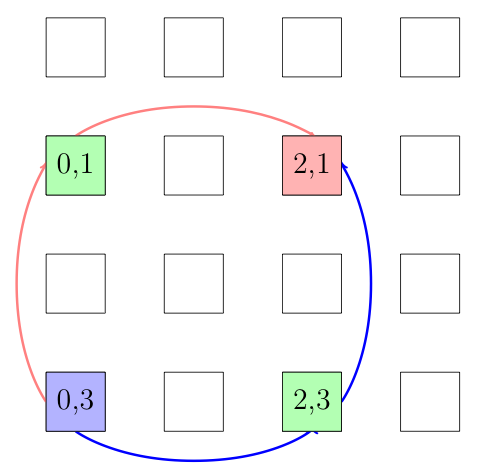
\includegraphics[width=0.5\textwidth]{figures/tikz/hypercube/hypercube_path.png}
\caption{Minimal routing within a hypercube showing path diversity. Packet travels from blue to red, passing through green intermediate switches.}
\label{fig:topologies:hypercubePath}
\end{figure}

To fully maximize path diversity on adversarial traffic patterns, though, path-diverse topologies can benefit from Valiant routing.
Here, rather than directly routing to the final destination, packets first route to random intermediate switches on a minimal path.
Then they route again from the intermediate switch to the final destination also on a minimal path (Figure \ref{fig:topologies:hypercubeValiant}).
Although it increases the hop count and therefore the point-to-point latency, it utilizes more paths and therefore increases the effective point-to-point bandwidth.

\begin{figure}[h!]
\centering
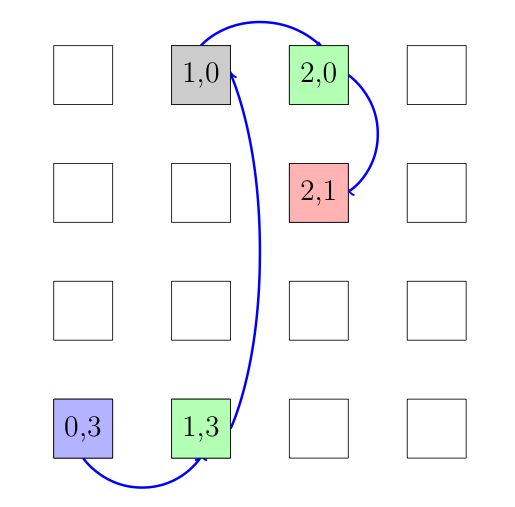
\includegraphics[width=0.5\textwidth]{figures/tikz/hypercube/hypercube_valiant.png}
\caption{Valiant routing within a hypercube.  Packet travels from blue to red via a random intermediate destination shown in gray. Additional intermediate switches are shown in green.}
\label{fig:topologies:hypercubeValiant}
\end{figure}

%% !TEX root = manual.tex

\section{Fat Tree}
\label{sec:tutorial:fattree}

Within SST, a fat tree is defined by the following parameters:

\begin{ViFile}
topology.name = fattree
topology.geometry = 4 2
\end{ViFile}
The first number, 4, indicates the number of levels in the fat tree.
The second number, 2, indicates the radix or branching factor of the tree.
The number of compute nodes in this topology is $2^4 = 16$.
This is illustrated conceptually in Figure \ref{fig:topologies:abstractfattree}.
The color coding will become clear later.
We note this is somewhat confusing since the fat tree appears to have 5 levels.
Here the topology is defined by the number of levels containing switches or the number of branches.
This is done for a very specific reason.  
At the final level, you may wish to have a different branching fraction for the compute nodes, e.g.

\begin{ViFile}
topology.concentration = 1
\end{ViFile}
This loads the injection bandwidth for the compute node dedicating its own injection switch.
If the parameter \inlineshell{network_nodes_per_switch} is omitted, it defaults to the fat tree radix.
This case is shown in Figure \ref{fig:topologies:abstractfattree} where there are two nodes injecting to the same switch.
Higher radix fat trees can be specified, e.g.

\begin{ViFile}
topology.name = fattree
topology.geometry = 3 4
\end{ViFile}
which would have $4^3 = 64$ compute nodes.

\begin{figure}[h!]
\centering
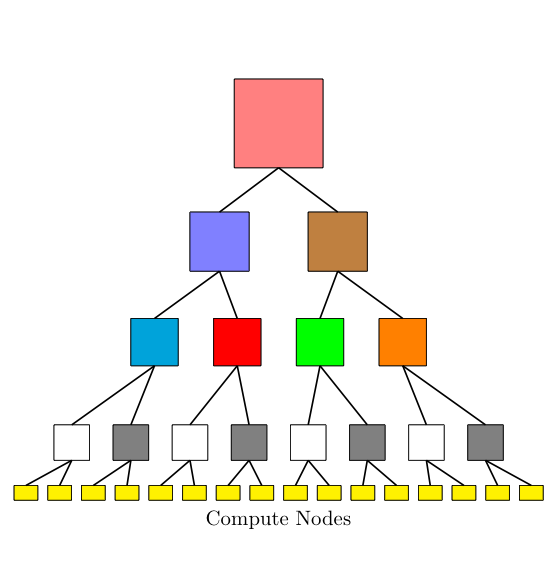
\includegraphics[width=0.9\textwidth]{figures/tikz/fattree/abstract_fattree.png}
\caption{Abstract, conceptual picture of Fat Tree topology}
\label{fig:topologies:abstractfattree}
\end{figure}

In reality, it is not practical to implement a fat tree exactly as shown in Figure \ref{fig:topologies:abstractfattree}.
One would need to buy many non-standard, high capacity switches for the higher levels in the fat-tree.
The simple model is available by specifying \inlineshell{simple_fattree} as the topology, and SST will construct special large switches at higher levels.
The best practical implementation employs all uniform, commodity switches (Figure \ref{fig:topologies:fattreeids}).
The fat tree is ``virtual'' with several commodity switches grouped together to simulate a heavy-weight, high capacity switch
at higher levels of the fat tree.
The connection between the physical implementation and the conceptual fat tree can easily be seen by the color coding.
For example, the second row contains eight switches, but only two virtual switches.
Each virtual switch is composed of four commodity switches.

\begin{figure}[h!]
\centering
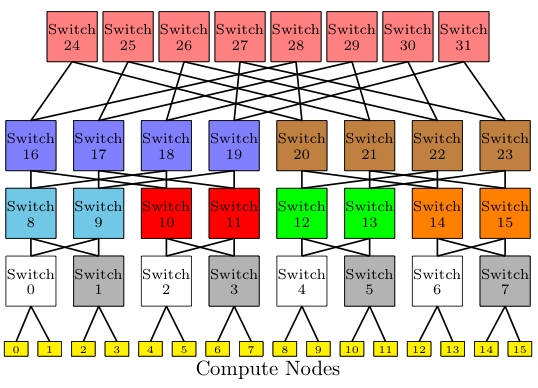
\includegraphics[width=0.9\textwidth]{figures/tikz/fattree/fattree_ids.png}
\caption{Physical implementation of Fat Tree with commodity switches showing ID numbering}
\label{fig:topologies:fattreeids}
\end{figure}

Within SST, each switch is assigned a unique ID, starting from zero in the bottom row and proceeding through the top level.
In addition, each compute node is also assigned a unique ID from 0 to 15.
The switches can also be defined by a set of coordinates.
While the choice of coordinate system for a 3D torus is obvious, 
the coordinate system for the fat tree is less clear.
In SST, we define a 2D mesh coordinate system for the row (level) and column of the switch.


\subsection{Allocation and indexing}
\label{subsec:fattree:allocation}
The numbering of compute nodes is shown in Figure \ref{fig:topologies:fattreeids}.
Consider the case

\begin{ViFile}
node.app1.launch_cmd = aprun -n 4 -N 1
\end{ViFile}
which launches four processes all on distinct nodes.
In the simplest allocation and indexing scheme (first available),
processes would be placed in order on 0,1,2,3.
An alternative allocation/indexing scheme uses the Node ID allocator.

\begin{ViFile}
node {
 app1 {
  allocation = node_id
  indexing = node_id
  node_id_file = nodes.txt
 }
}
\end{ViFile}
Here \inlineshell{nodes.txt} would contain the number of nodes on the first line, followed by the list of Node IDs, in order, of where to place MPI ranks.
For the file

\begin{ViFile}
4
0
4
8
12
\end{ViFile}
Four MPI ranks would be placed in spatially distant parts of the machine.

If indexing differs from allocation (usually because there are multiple MPI ranks per node), both an allocation and an indexing file are needed.
Suppose we have:

\begin{ViFile}
node.app1.launch_cmd = aprun -n 4 -N 2
\end{ViFile}
We then need:

\begin{ViFile}
node {
 app1 {
  allocation = node_id
  indexing = node_id
  node_id_allocation_file = alloc.txt
  node_id_indexing_file = index.txt
 }
}
\end{ViFile}
where the contents of \inlineshell{alloc.txt} are, e.g.

\begin{ViFile}
2
0
1
\end{ViFile}
choosing nodes 0 and 1 in the allocation and then \inlineshell{index.txt} would be, e.g.

\begin{ViFile}
4
0
1
0
1
\end{ViFile}
which round-robin assigns rank 0 to node, rank 1 to node 1, rank 2 to node 0, and so on.

\subsection{Routing}
\label{subsec:fattree:routing}

Fat tree routing is actually straightforward, but can employ path diversity.
Suppose you are routing from Node 0 to Node 2 (Figure \ref{fig:topologies:fattreeids}).
At the first stage, you have no choice.
You must route to Switch 1.
At the second stage, you can either route to Switch 8 or Switch 9.
Suppose you branch to Switch 9. 
At this point, you are done moving up.
The packet now proceeds down the fat-tree.
On the downward routing, there is no path diversity.
Only a single, minimal route exists to the destination node.
In the simplest case, Switch 1 alternates between selecting Switch 8 and Switch 9 to distribute load.
In a more complicated scheme, Switch 1 could adaptively route selecting either Switch 8 or Switch 9 based on congestion information.

%% !TEX root = manual.tex

\section{Dragonfly}
\label{sec:tutorial:dragonfly}

\begin{figure}[h!]
\centering
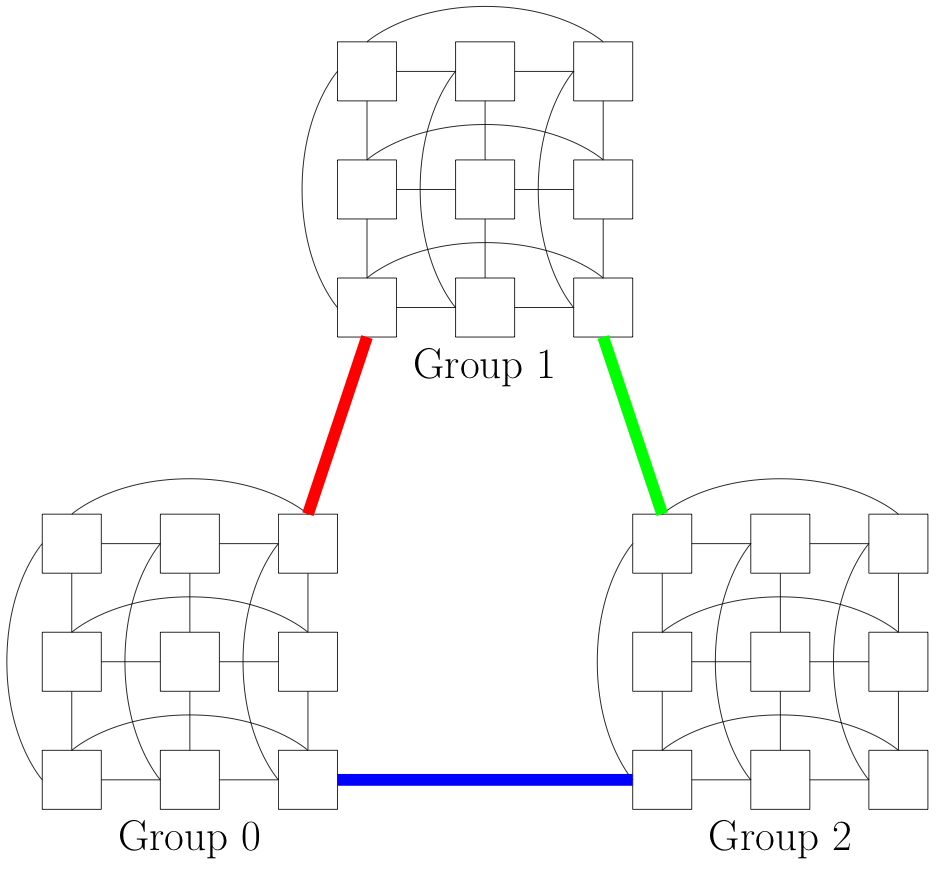
\includegraphics[width=0.7\textwidth]{figures/tikz/dragonfly/dragonfly.png}
\caption{Schematic of dragonfly with three groups showing hypercube intragroup links and high bandwidth intergroup global links}
\label{fig:topologies:dragonfly}
\end{figure}

As bandwidth per pin increases, arguments can be made that optimal topologies should be higher radix.
A 3D torus is on the low-radix extreme while a hypercube is a high-radix extreme.
Unfortunately a hypercube topology is not scalable and the radix quickly becomes too high to efficiently implement.
A dragonfly is sometimes viewed as a generalization of flattened butterfly and hypercube topologies with ``virtual'' switches of very high radix,
not dissimilar from the fat-tree implementation with many physical commodity switches composing a single virtual switch.
The dragonfly topology (Figure \ref{fig:topologies:dragonfly}) is actually quite simple. 
Small groups are connected as a generalized hypercube with full connectivity within a row or column.
Intergroup connections (global links) provide pathways for hopping between groups.
A dragonfly is usually understood through three parameters:
\begin{itemize}
\item $p$: number of nodes connected to each router
\item $a$: number of routers in a group
\item $h$: number of global links that each switch has
\end{itemize}

For simplicity, only three example global links are show for clarity in the picture.
For the Cray X630, $a = 96$, $h=10$, and $p=4$ so that each router is connected to many other ($h=10$) groups.
The caveat is that in many implementations global links are grouped together for $h=2$ or $3$ fat global links.
These demonstrate well-balanced ratios.
In general, scaling out a dragonfly should not increase the size of a group, only the number of groups.

\subsection{Allocation and indexing}
\label{subsec:dragonfly:allocatoin}

The dragonfly coordinate system is essentially the same as a 3D torus.  
The group 2D hypercube layout defines $X$ and $Y$ coordinates.
The group number defines a $Z$ or $G$ coordinate.
Thus the topology in Figure \ref{fig:topologies:dragonfly} would be specified as

\begin{ViFile}
topology.name = dragonfly
topology.geometry = 3 3 3
\end{ViFile}
for groups of size $3 \times 3$ with a total of 3 groups.
To complete the specification, the number of global links ($h$) for each router must be given

\begin{ViFile}
topology.group_connections = 10
\end{ViFile}

\subsection{Routing}
\label{subsec:dragonfly:routing}

It is important to understand the distinction between link bandwidth, channel bandwidth, and pin bandwidth.
All topologies have the same pin bandwidth and channel bandwidth (assuming they use the same technology).
Each router in a topology is constrained to have the same number of channels (called radix, usually about $k=64$).
The number of channels per link changes dramatically from topology to topology.
Low radix topologies like 3D torus can allocate more channels per link, 
giving higher bandwidth between adjacent routers.
Dragonfly is higher radix, having many more connections but having lower bandwidth between adjacent routers.
While minimal routing is often sufficient on torus topologies because of the high link bandwidth,
dragonfly will exhibit very poor performance with minimal routing.
To effectively utilize all the available bandwidth, packets should have a high amount of path diversity.
Packets sent between two routers should take as many different paths as possible to maximize the effective bandwidth point-to-point.

\begin{figure}[h!]
\centering
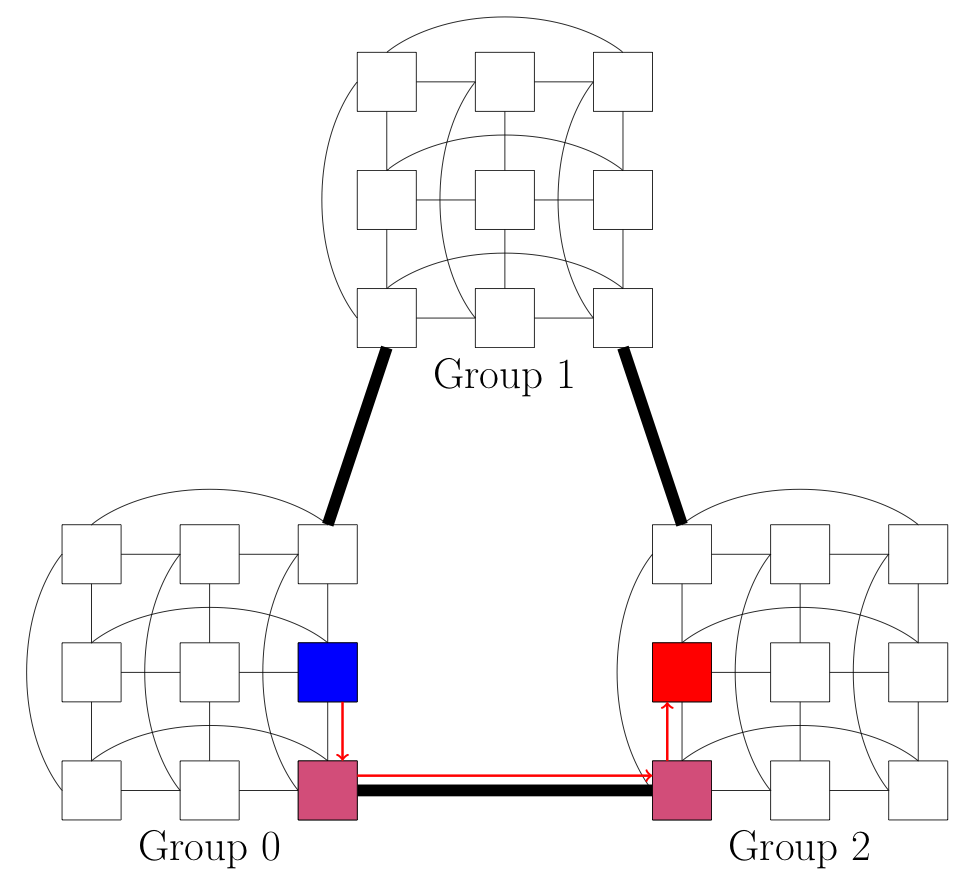
\includegraphics[width=0.7\textwidth]{figures/tikz/dragonfly/dflyminroute.png}
\caption{Schematic of dragonfly showing minimal route. Traveling between groups requires routing to the correct global link, hopping the global link, then routing within a group to the correct final node.}
\label{fig:topologies:dflyminroute}
\end{figure}

Minimal routing itself has a few complications (Figure \ref{fig:topologies:dflyminroute}).  
Each router only has a few global links.  
Thus, traveling from e.g. the blue router at X=3,Y=2,G=0 to the red router at X=1,Y=2,G=2, there is no direct link between the routers.
Furthermore, there is no direct link between Groups 0 and 2.
Thus packets must route through the purple intermediate nodes.
First, the packet hops to X=3,Y=3, G=0.  
This router has a global link to Group 2, allowing the packet to hop to the next intermediate router at X=1, Y=3, G=2.
Finally, the minimal route completes by hopping within Group 2 to the final destination.

\begin{figure}[h!]
\centering
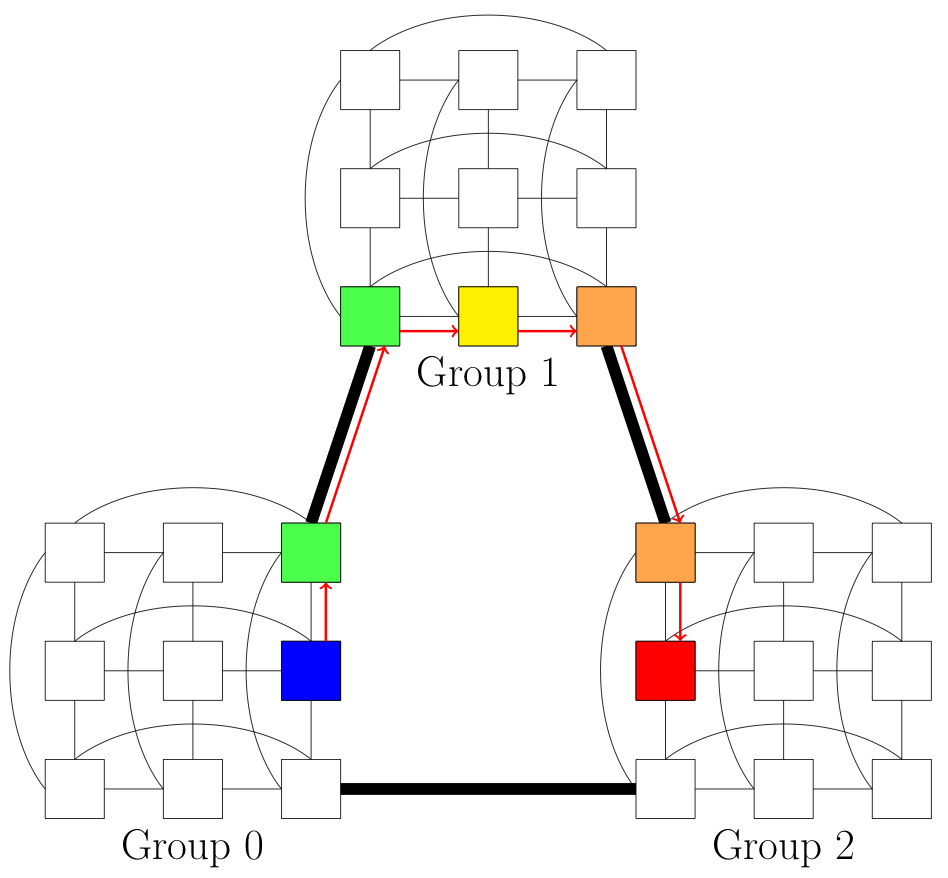
\includegraphics[width=0.7\textwidth]{figures/tikz/dragonfly/dflyvaliant.png}
\caption{Schematic of dragonfly showing Valiant route. Traveling between groups requires routing to a random intermediate node, then routing minimally to the final destination.}
\label{fig:topologies:dflyvaliantroute}
\end{figure}

To improve on minimal routing, global routing strategies are required (global routing is distinguished here from adaptive routing).  
Global essentially means ``not minimal'' and spreads packets along many different paths.
The simplest global routing strategy is Valiant routing, which falls in the global, oblivious category (Figure \ref{fig:topologies:dflyvaliantroute}).
Oblivious simply means packets are scattered randomly without measuring congestion.
In Valiant routing, each packet does the following:
\begin{itemize}
\item Pick a random intermediate node 
\item Route minimally to random node
\item Route minimally from random node to destination node
\end{itemize}
This is somewhat counterintuitive at first.
Rather than go directly to the destination node, packets go out of their way to a random node, shown in Figure \ref{fig:topologies:dflyvaliantroute} as the yellow router.
Thus, routing from the blue router in Group 0 to the red router in Group 2 first follows the minimal path (green routers) to the randomly selected yellow router in Group 1. 
From there, a second minimal path is taken through the orange routers to the final destination.
In cases with high congestion or even for large messages on a quiet network, this actually improves performance.
If a point-to-point message is composed of ten packets,
all ten packets will follow different paths to the final destination.
This essentially multiplies the maximum bandwidth by a factor of ten.
Valiant routing can be specified as

\begin{ViFile}
router = valiant
\end{ViFile}

In contrast, UGAL routing is a global, adaptive strategy, making decisions based on congestion.
Because Valiant is oblivious, it often sends too many packets to far away random nodes.
Following a Valiant path is only relevant when enough packets fill up router queues, creating congestion.
UGAL does the following steps:
\begin{itemize}
\item Start routing minimally
\item On each step, check congestion (buffer queue depth)
\item If congestion is too heavy, switch to Valiant and re-route to random intermediate node. Otherwise stay on minimal path.
\end{itemize}
UGAL packets stay on a minimal path until congestion forces them to use a Valiant strategy.
This routing can be specified as:

\begin{ViFile}
router = ugal
\end{ViFile}




